\documentclass[aspectratio=1610,17pt,utf8]{beamer}

\usepackage[utf8]{inputenc}
\usepackage[T1]{fontenc}
%\usepackage[USenglish]{babel}
%\usepackage[latin1]{inputenc}
\usepackage[frenchb]{babel}
\usepackage{graphicx} % graphics
\usepackage{mathabx}
\usepackage{mathpazo}
\usepackage{eulervm}

\usepackage{amsmath}
\usepackage{amssymb} % not along with newtxmath
\usepackage{amsthm}
%\usepackage{bm}

\usepackage{adjustbox}
\usepackage{xcolor,colortbl}

\definecolor{rougePire}{rgb}{230,65,65}
\definecolor{vertMieux}{rgb}{123,220,104}

\newcolumntype{p}{>{\columncolor{rougePire}}c}
\newcolumntype{m}{>{\columncolor{vertMieux}}c}

\newcommand{\N}{\mathbb{N}}
\newcommand{\Z}{\mathbb{Z}}
\newcommand{\R}{\mathbb{R}}
\newcommand{\E}{\mathbb{E}}
\newcommand{\Pb}{\mathbb{P}}
\newcommand{\deriv}{\mathrm{d}}
\newcommand{\A}{\mathcal{A}}
\newcommand{\Un}{\mathds{1}}
\newcommand{\Sy}{\mathbb{S}}

\theoremstyle{definition}
\newtheorem*{theo}{Théorème}

%\usepackage{helvet}
\usefonttheme{professionalfonts}
\usepackage[sfdefault,light,condensed]{roboto}
%\usepackage[sfdefault,lf]{carlito}
%\usepackage{uarial}

\setbeamercolor{math text}{fg=black!15!uidarkred}

%\usetheme{Pittsburgh}
%\usetheme{unipassau}
%\usetheme{hsrm}
%\usetheme{samone}
%\usetheme{samtwo}
\usetheme{samthree}

% title slide definition
%\title[Shorter Title]{Title of the Presentation}
\title[Online Convex Optimization]{Optimisation convexe en ligne}
%\subtitle{Subtitle}
\subtitle{Regrets logarithmiques}
%\author[Shorter Author]{Complete Author list}
\author[Givois - Sall]{Samuel Givois - Fatou Sall}
\institute[Ensae]
{
  Apprentissage en ligne\\
  Ensae\\
}
\date{Vendredi 6 avril 2018}

%--------------------------------------------------------------------
%                            Page de titre
%--------------------------------------------------------------------

\begin{document}

\begin{frame}[plain]
  \titlepage
\end{frame}

\begin{frame}[plain]
  \tableofcontents
\end{frame}

%-------------------------------------------------------------------
%                            Problème
%-------------------------------------------------------------------
\section{Problème}

\begin{frame}{Objectif}

{\footnotesize Hazan, E., Kalai, A., Kale, S., Agarwal, A. (2006, June). Logarithmic regret algorithms for online convex optimization. \textit{International Conference on Computational Learning Theory} (pp. 499-513). Springer, Berlin, Heidelberg.}

\begin{itemize}
    \item Problème d'optimisation convexe en ligne.
    \item Cadre introduit par Zinkevich en 2003.
    \begin{itemize}
        \item Descente de gradient en ligne en $O(\sqrt{T})$
    \end{itemize}
    \item Algorithmes en $O(\log(T))$ sous certaines hypothèses
\end{itemize}

\end{frame}

\begin{frame}{Croissances des bornes}
    
\begin{figure}[H]
    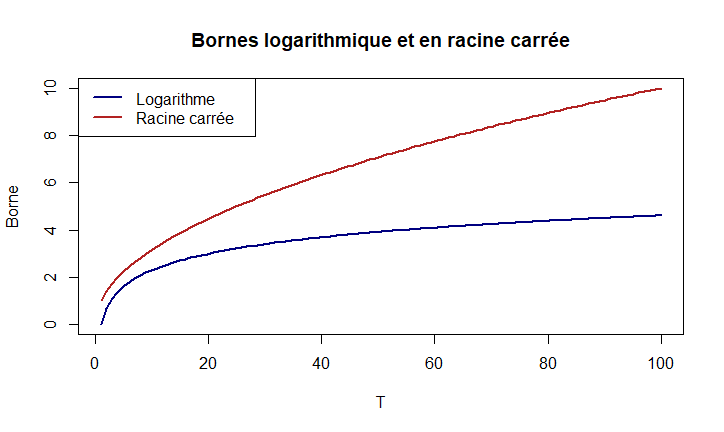
\includegraphics[width=0.85\textwidth]{img/borne_log_racine.png}
\end{figure}

\end{frame}

\begin{frame}{Notations}

\begin{itemize}
    \item Ensemble convexe $K \in \R^n$
    \item $T$ périodes
    \item Décisions $x_1, ..., x_T \in K$
    \item Fonctions de perte convexes $f_1, ..., f_T : K \rightarrow \R$
\end{itemize}

Regret : $R_T = \sum\limits_{t=1}^T f_t(x_t) - \underset{x \in K}{\text{min}} \sum\limits_{t=1}^T f_t(x)$

On veut garantir $R_T$ faible

\end{frame}

%-------------------------------------------------------------------
%                            Hypothèses
%-------------------------------------------------------------------
\section{Hypothèses}

\begin{frame}{Hypothèses}

Hypothèse forte :
\begin{itemize}
    \item $G \geq 0$ : $\exists G \geq 0$ tq $\forall t \leq T$, $\forall x \in K$, $||\nabla f_t(x)|| \leq G$
    \item $H \geq 0$ : $\exists H \geq 0$ tq $\forall t \leq T$, $\forall x \in K$, $\nabla^2 f_t(x) \succeq H I_n$
\end{itemize}

Hypothèse faible :
\[ \exists \alpha \geq 0 \text{ tq } \forall t \leq T, h_t : x \mapsto e^{-\alpha f_t(x)} \text{ est concave sur } K \]
La première implique la seconde.

\end{frame}

\begin{frame}{Démonstration}

Démonstration en dimension 1 :
\[
\begin{array}{c}
h_t''(x) = ((\alpha f_t'(x))^2 - \alpha f_t''(x))e^{-\alpha f_t(x)} \leq 0 \\
\Longleftrightarrow \\
\alpha \leq \frac{f_t''(x)}{(f_t'(x))^2}
\end{array}
\]

\end{frame}

\begin{frame}{Résultats}

A remplir

\end{frame}

%-------------------------------------------------------------------
%                            OGD et EWOO
%-------------------------------------------------------------------
\section{OGD et EWOO}

\begin{frame}{Descente de gradient en ligne (OGD)}

Descente de gradient dans le cadre \og en ligne\fg. 

Pas : $\eta_1, ..., \eta_T$.

Mise à jour :
\[
x_{t+1} = \Pi_K(x_t - \eta_{t+1} \nabla f_t (x_t))
\]
Projection :
\[
\Pi_K(y) = \underset{x \in K}{\text{argmin}} ||x-y||
\]
    
\end{frame}

\begin{frame}{OGD - Borne du regret}

\begin{theo}
Supposons que $\exists G, H \geq 0$ tel que $\forall t \leq T$, $\forall x \in K$, $||\nabla f_t(x)|| \leq G$ et $\nabla^2f_t(x) \succeq HI_n$.

Alors, en prenant $\forall t \leq T$, $\eta_t = \frac{1}{Ht}$, on a :
\[
R_T \leq \frac{G^2}{2H}(1 + \log(T))
\]
\end{theo} 

\end{frame}

\begin{frame}{OGD - Eléments de preuve}

\begin{enumerate}
    \item Inégalité de Taylor-Lagrange :
    
    $f_t(x_t) - f_t(x^*) \leq \nabla_t^T(x_t - x^*) - \frac{H}{2}||x^* - x_t||^2$
    \item Propriété des projections sur un ensemble convexe :
    
    borne pour $\nabla_t^T(x_t - x^*)$
    \item Simplification grâce au choix des $\eta_t$
\end{enumerate}

\end{frame}

\begin{frame}{Poids exponentiels (EWOO)}

Généralisation de l'algorithme $EWA$ au cas continu.

Poids exponentiels :
\[
w_{t+1}(x) = e^{-\alpha\sum\limits_{\tau = 1}^{t} f_{\tau}(x)} = \prod\limits_{\tau = 1}^{t} h_{\tau}(x)
\]
Mise à jour :
\[
x_{t+1} = \frac{\int_K x w_{t+1}(x)\deriv x}{\int_K w_{t+1}(x)\deriv x}
\]
    
\end{frame}

\begin{frame}{EWOO - Borne du regret}

\begin{theo}
Supposons que $\exists \alpha$ tel que $\forall t\leq T$, $h_t : x \mapsto e^{-\alpha f_t(x)}$ est concave sur $K$.

Alors, on a :
\[
R_T \leq \frac{n}{\alpha}(1 + \log(1 + T))
\]
\end{theo}

\end{frame}

\begin{frame}{EWOO - Eléments de preuve}

\begin{enumerate}
    \item Concavité de $h_t$ et inégalité de Jensen, puis produit téléscopique : $\prod\limits_{\tau = 1}^t h_{\tau}(x_{\tau}) \geq \frac{\int_K \prod\limits_{\tau = 1}^t h_{\tau}(x) \deriv x}{\text{vol}(K)}$
    \item Borne sur ensemble $S$ construit à partir de $x^*$ et $K$ (concavité et positivité de $h_t$).
    \item Volume de $S$ à partir de celui de $K$ (mise à l'échelle en dimension $n$).
\end{enumerate}

\end{frame}

%-------------------------------------------------------------------
%                            Online Newton Step
%-------------------------------------------------------------------
\section{\og Online Newton Step\fg}

%-------------------------------------------------------------------
%                            Implémentation
%-------------------------------------------------------------------
\section{Implémentation}

\end{document}
